\begin{name}
	{\tenchude}
	{ĐỀ ÔN TẬP CHƯƠNG I}
	{LỚP TOÁN THẦY PHÁT}
	{\thoigian}
\end{name}
\TN
\Opensolutionfile{ans}[ans/ans\currfilebase-Phan-I]
\begin{ex}%[2-D1B5-SO-15-2425]%[VN-MT-7, Đoàn Thị Lý]%[2D1N1-1]
 Cho hàm số $y=f(x)$ có đạo hàm $f'(x)=x(x-2)^3$, với mọi $x \in \mathbb{R}$. Hàm số đã cho nghịch biến trên khoảng nào dưới đây?
 \choice 
 {$(1;3)$}
 {$(-1;0)$}
 {\True $(0;1)$}
 {$(-2;0)$}
 \loigiai{
 Ta có $f'(x)=0 \Leftrightarrow\hoac{&x=0 \\&x=2.}$ \\
 Bảng xét dấu $f'(x)$
 \begin{center}
 
\begin{tikzpicture}
 \tkzTabInit[nocadre=true,lgt=1.2,espcl=2.5,deltacl=0.5]
 {$x$ /.7, $f'(x)$ /.7}
 {$-\infty$,$0$,$2$,$+\infty$}
 \tkzTabLine{ ,+,0,-,0, +, }
 \end{tikzpicture}
 \end{center}
 Dựa vào bảng xét dấu $f'(x)$ ta thấy hàm số đã cho nghịch biến trên $(0;1)$.
 }
\end{ex}

\begin{ex}%[2-D1B5-SO-15-2425]%[VN-MT-7, Đoàn Thị Lý]%[2D1N1-2] 
 Cho hàm số $y=f(x)$ có tập xác định là $\mathscr{D}=\mathbb{R}\setminus\big\{-1\big\}$ và có bảng xét dấu của đạo hàm như hình sau:
 \begin{center}
 
\begin{tikzpicture}
 \tkzTabInit[nocadre=true,lgt=1.2,espcl=2.5,deltacl=0.5]
 {$x$ /.7, $f'(x)$ /.7}
 {$-\infty$,$-1$,$1$,$+\infty$}
 \tkzTabLine{ ,-,d,-,0, +, }
 \end{tikzpicture}
 \end{center}
 Hàm số đã cho nghịch biến trên khoảng nào dưới đây? 
 \choice 
 {$(1 ;+\infty)$}
 {$(-\infty; 1)$}
 {$(-1;+\infty)$}
 {\True $(-\infty;-1)$}
 \loigiai{ 
 Từ bảng xét dấu ta thấy hàm số đã cho nghịch biến trên khoảng $(-\infty;-1)$.
 }
\end{ex}

\begin{ex}%[2-D1B5-SO-15-2425]%[VN-MT-7, Đoàn Thị Lý]%[2D1N3-1]
 \immini{
 Cho hàm số $y=f(x)$ liên tục trên đoạn $[-2;2]$ và có đồ thị như hình vẽ bên. Gọi $M$ và $m$ lần lượt là giá trị lớn nhất và giá trị nhỏ nhất của hàm số đã cho trên đoạn $[-2;2]$. Giá trị của $M+m$ bằng
 \choice[2]
 {$0$}
 {$1$}
 {$4$}
 {\True $3$}
 }
 {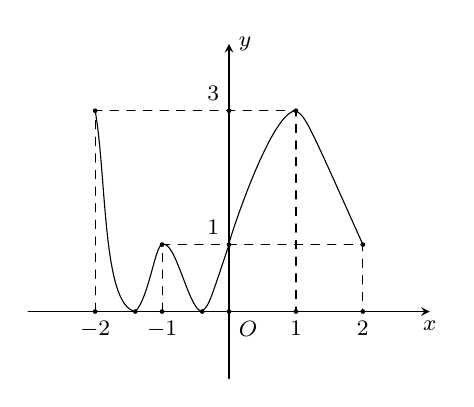
\begin{tikzpicture} [scale=.85, font=\footnotesize, line join=round, line cap=round, >=stealth]
 \draw[->] (-3,0)--(0,0) node[below right]{$O$}--(3,0) node[below]{$x$};
 \draw[->] (0,-1)--(0,4) node[right]{$y$};
 \draw (-2,3) .. controls ++(-80:1) and ++(170:.5) .. (-1.4,0).. controls (-1.2,.2) and (-1.1,1).. (-1,1).. controls (-.8,1.1) and (-.6,0) .. (-.4,0) .. controls (-.3,0.1) .. (0,1).. controls (-.1,.75) and (.6,3) .. (1,3).. controls (1.15,2.9).. (2,1);
 \draw[dashed] (-2,0) node[below]{$-2$}--(-2,3) --(0,3)node[above left]{$3$}--(1,3)--(1,0)node[below]{$1$} (-1,0)node[below]{$-1$}--(-1,1)--(0,1)node[above left]{$1$}--(2,1)--(2,0)node[below]{$2$};
 \foreach \i in {(0,3),(-2,3),(1,3),(-1,1),(0,1),(-2,0), (-1,0),(1,0),(2,0),(2,1),(-1.4,0),(-.4,0),(0,0)}\fill \i circle (1pt); 
 \end{tikzpicture}
 }
 \loigiai{ 
 Quan sát đồ thị ta thấy $M=\max\limits_{[-2;2]} f(x)=3$ và $m=\min\limits_{[-2 ; 2]} f(x)=0$. Vậy $M+m=3+0=3$.
 }
\end{ex}

\begin{ex}%[2-D1B5-SO-15-2425]%[VN-MT-7, Đoàn Thị Lý]%[2D1N4-1]
 Cho hàm số $y=f(x)$ có bảng biến thiên như sau:
 \begin{center}
 
\begin{tikzpicture}
 \tkzTabInit[nocadre=true,lgt=1.2,espcl=3, deltacl=0.5]
 {$x$/0.7,$f’(x)$/0.7,$f(x)$/2}
 {$-\infty$,$0$,$1$,$+\infty$}
 \tkzTabLine{,+,0,-,d,+,}
 \tkzTabVar{-/$0$,+/$2$,-D-/$-\infty$/$3$,+/$5$}
 \end{tikzpicture}
 \end{center}
 Tổng số tiệm cận ngang và tiệm cận đứng của đồ thị hàm số đã cho là 
 \choice 
 {$4$}
 {\True $3$}
 {$2$}
 {$1$}
 \loigiai{
 Từ bảng biến thiên ta có
 \begin{itemize}
 \item $\lim\limits _{x \to-\infty} y=0$, suy ra đồ thị hàm số có tiệm cận ngang là $y=0$.
 \item $\lim\limits _{x\to+\infty} y=5$, suy ra đồ thị hàm số có tiệm cận ngang là $y=5$.
 \item $\lim\limits _{x \to 1^-} y=+\infty$, suy ra đồ thị hàm số có tiệm cận đứng là $x=1$.
 \end{itemize}
 Vậy tổng số tiệm cận ngang và tiệm cận đứng của đồ thị hàm số đã cho là $3$.
 }
\end{ex}

\begin{ex}%[2-D1B5-SO-15-2425]%[VN-MT-7, Đoàn Thị Lý]%[2D1N4-1]
 Cho hàm số $y=\dfrac{2 x+1}{x-3}$. Tiệm cận ngang của đồ thị hàm số đã cho là
 \choice 
 {$x=3$}
 {$x=2$}
 {$x=-\dfrac{1}{2}$}
 {\True $y=2$}
 \loigiai{
 Ta có $\lim\limits _{x \to \pm \infty} y=\lim\limits _{x \to \pm \infty} \dfrac{2 x+1}{x-3}=\lim\limits _{x \to \pm \infty} \dfrac{2+\dfrac{1}{x}}{1-\dfrac{3}{x}}=2$, suy ra đồ thị hàm số có tiệm cận ngang $y=2$.
 }
\end{ex}

\begin{ex}%[2-D1B5-SO-15-2425]%[VN-MT-7, Đoàn Thị Lý]%[2D1N5-1]
 \immini{
 Biết hàm số $y=\dfrac{ax+b}{cx+d}$ có đồ thị như trong hình vẽ bên. Mệnh đề nào dưới đây đúng?
 \choice
 {\True $y'>0$, $\forall x \neq 1$}
 {$y'>0$, $\forall x \in \mathbb{R}$}
 {$y'<0$, $\forall x \in \mathbb{R}$}
 {$y'<0$, $\forall x \neq 1$}
 }{
 \begin{tikzpicture} [scale=.8, font=\footnotesize, line join=round, line cap=round, >=stealth]
 \draw[->] (-2,0)--(0,0) node[below right]{$O$}--(1,0) node[above right]{$1$}--(4,0) node[below]{$x$}; 
 \draw[->] (0,-2)--(0,4) node[left]{$y$}; 
 \fill (0,0) circle (1.0pt) (1,0) circle (1.0pt); 
 \begin{scope}
 \clip (-2,-2) rectangle (4,4);
 \draw[samples=300,domain=-2:4,smooth] plot (\x, {(\x-2)/(\x-1)}); 
 \end{scope}
 \draw (-2,1)--(4,1); 
 \end{tikzpicture}
 }
 \loigiai{ 
 Tập xác định của hàm số đã cho là $\mathscr{D}=\mathbb{R}\setminus\{1\}$.\\
 Từ đồ thị của hàm số suy ra hàm số đã cho đồng biến trên mỗi khoảng xác định vì vậy $y'>0, \forall x \neq 1$.
 }
\end{ex}

\begin{ex}%[2-D1B5-SO-15-2425]%[VN-MT-7, Đoàn Thị Lý]%[2D1N5-1]
 \immini{Đồ thị của hàm số nào dưới đây có dạng như đường cong trong hình bên?
 \choice 
 {\True $y=x^3-3 x$}
 {$y=-x^3+3 x$}
 {$y=x^4-2 x^2$}
 {$y=-x^4+2 x^2$}
 }
 {
 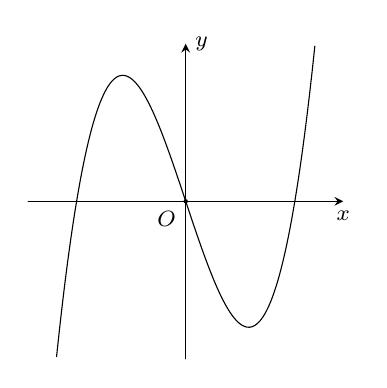
\begin{tikzpicture} [scale=.8, font=\footnotesize, line join=round, line cap=round, >=stealth]
 \draw[->] (-2.5,0)--(0,0) node[below left]{$O$}--(2.5,0) node[below]{$x$};
 \draw[->] (0,-2.5)--(0,2.5) node[right]{$y$};
 \draw[samples=100,domain=-2.05:2.05,smooth] plot (\x, {(\x)^3-3*(\x)});
 \fill (0,0) circle (1.0pt);
 \end{tikzpicture} 
 }
 \loigiai{
 Đường cong có dạng của đồ thị hàm số bậc ba với hệ số $a>0$ nên chỉ có hàm số $y=x^3-3 x$ thỏa yêu cầu bài toán.
 }
\end{ex}

\begin{ex}%[2-D1B5-SO-15-2425]%[VN-MT-7, Đoàn Thị Lý]%[2D1H1-3]
 Tập hợp tất cả các giá trị thực của tham số $m$ để hàm số $y=x^3+(m+1) x^2+3 x+2$ đồng biến trên $\mathbb{R}$ là
 \choice 
 {\True $[-4;2]$}
 {$(-4;2)$}
 {$(-\infty;-4] \cup[2;+\infty)$}
 {$(-\infty;-4)\cup(2;+\infty)$}
 \loigiai{ 
 Tập xác định $\mathscr{D}=\mathbb{R}$.\\
 Ta có $y'=3 x^2+2(m+1) x+3$.\\
 Hàm số $y=x^3+(m+1) x^2+3 x+2$ đồng biến trên $\mathbb{R}$ khi và chỉ khi 
 \[y' \geq 0, \forall x \in \mathbb{R}
 \Leftrightarrow \Delta'=(m+1)^2-9 \leq 0 \Leftrightarrow m^2+2 m-8 \leq 0 \Leftrightarrow-4 \leq m \leq 2.\] 
 Vậy $m \in[-4 ; 2]$.
 }
\end{ex}

\begin{ex}%[2-D1B5-SO-15-2425]%[VN-MT-7, Đoàn Thị Lý]%[2D1H3-1]
 Gọi $M$ và $m$ lần lượt là giá trị lớn nhất và giá trị nhỏ nhất của hàm số $y=f(x)=\dfrac{2x+1}{x-2}$ trên đoạn $[3;7]$ . Tính giá trị của $M^2+m$.
 \choice 
 {\True $52$}
 {$58$}
 {$6$}
 {$10$}
 \loigiai{
 Hàm số $y=f(x)=\dfrac{2 x+1}{x-2}$ liên tục trên $[3;7]$.\\
 Ta có 
 $y'=\dfrac{-5}{(x-2)^2}<0, \forall x \in[3 ; 7]$ nên hàm số $y=f(x)$ nghịch biến trên $[3;7]$.\\ Lúc đó
 \[M=\max\limits_{[3;7]} f(x) = f(3)=7,m=\min\limits_{[3;7]}f(x)=f(7)=3.\]
 Vậy $M^2+m=52$.
 }
\end{ex}

\begin{ex}%[2-D1B5-SO-15-2425]%[VN-MT-7, Đoàn Thị Lý]%[2D1H4-1]
 Đồ thị hàm số $y=\dfrac{x^2-3 x-4}{x^2-16}$ có bao nhiêu đường tiệm cận đứng? 
 \choice 
 {\True $1$}
 {$0$}
 {$2$}
 {$3$}
 \loigiai{
 Tập xác định $\mathscr{D}=\mathbb{R} \setminus\big\{- 4;4\big\}$. Ta có
 \begin{itemize}
 \item $\lim\limits _{x \to (-4)^-} y=\lim\limits _{x \to (-4)^-} \dfrac{x^2-3 x-4}{x^2-16}=\lim\limits _{x \to (-4)^-} \dfrac{(x+1)(x-4)}{(x+4)(x-4)}=\lim\limits _{x \to (-4)^-} \dfrac{x+1}{x+4}=+\infty$, suy ra $x=-4$ là tiệm cận đứng của đồ thị hàm số.
 \item $\lim\limits_{x \to 4} y=\lim\limits _{x \to 4} \dfrac{x^2-3 x-4}{x^2-16}=\lim\limits _{x \to 4} \dfrac{(x+1)(x-4)}{(x+4)(x-4)}=\lim\limits _{x \to 4} \dfrac{x+1}{x+4}=\dfrac{5}{8}$, suy ra $x=4$ không là tiệm cận đứng của đồ thị hàm số.
 \end{itemize}
 Vậy đồ thị hàm số có $1$ đường tiệm cận đứng.
 }
\end{ex}

\begin{ex}%[2-D1B5-SO-15-2425]%[VN-MT-7, Đoàn Thị Lý]%[2D1H5-4] 
 Đồ thị của hàm số $y=x^3-3 x+2$ cắt trục tung tại điểm có tung độ bằng 
 \choice
 {$0$}
 {$1$}
 {\True $2$}
 {$3$}
 \loigiai{
 Gọi $M\left(x_0;y_0\right)$ là giao điểm của đồ thị hàm số với trục tung. Ta có $x_0=0 \Rightarrow y_0=2$.
 }
\end{ex}

\begin{ex}%[2-D1B5-SO-15-2425]%[VN-MT-7, Đoàn Thị Lý]%[2D1H5-4]
 Số giao điểm của đồ thị hàm số $y=x^3-3 x+1$ và trục hoành là \choice 
 {\True $3$}
 {$0$}
 {$2$}
 {$1$}
 \loigiai{
 Tập xác định $\mathscr{D}=\mathbb{R}$.\\
 Ta có $y'=3 x^2-3=3\left(x^2-1\right)$, $y'=0 \Leftrightarrow x= \pm 1$.\\
 Bảng biến thiên của hàm số
 \begin{center}
 
\begin{tikzpicture}
 \tkzTabInit[nocadre=true,lgt=1.2,espcl=3, deltacl=0.5]
 {$x$/0.7,$y'$/0.7,$y$/2}
 {$-\infty$,$-1$,$1$,$+\infty$}
 \tkzTabLine{,-,0,+,0,-,}
 \tkzTabVar{-/$-\infty$,+/$3$,-/$-1$,+/$+\infty$}
 \end{tikzpicture}
 \end{center}
 Từ bảng biến thiên ta thấy đồ thị hàm số cắt trục hoành tại $3$ điểm phân biệt.
 }
\end{ex}
\Closesolutionfile{ans}

\TNTF
\Opensolutionfile{ans}[ans/ans\currfilebase-Phan-II]
\begin{ex}%[2-D1B5-SO-15-2425]%[VN-MT-7, Đoàn Thị Lý]%[2D1N3-1]
 \immini{
 Cho hàm số $y=f(x)$ liên tục trên $\mathbb{R}$ và có đồ thị như hình vẽ bên. 
 \choiceTF
 {\True Hàm số đồng biến trên khoảng $(0;2)$}
 {Hàm số đạt cực đại tại $x=0$}
 {\True Giá trị nhỏ nhất của hàm số trên $[-1;1]$ bằng $-4$} 
 {Hàm số $g(x)=f(3-x)$ nghịch biến trên $(2;5)$}
 }
 {
 \begin{tikzpicture} [scale=.8, font=\footnotesize, line join=round, line cap=round, >=stealth]
 \draw[->] (-1.8,0)--(-1,0) node[below left]{$-1$}--(0,0) node[below left]{$O$}--(2,0) node[above]{$2$}--(3.2,0) node[below]{$x$};
 \draw[->] (0,-4.8)--(0,-4) node[below left]{$-4$}--(0,1.2) node[right]{$y$};
 \draw[samples=100,domain=-1.1:3.05,smooth] plot (\x, {-(\x)^3+3*(\x)^2-4});
 \foreach \x in {(0,0),(-1,0),(0,-4),(2,0)}
 \fill \x circle (1pt);
 \end{tikzpicture}
 }
 \loigiai{
 \begin{itemchoice}
 \itemch \textbf{Đúng}.\\
 Hàm số đồng biến trên khoảng $(0;2)$.
 \itemch \textbf{Sai}.\\
 Hàm số đạt cực đại tại $x=2$.
 \itemch \textbf{Đúng}.\\
 Ta có $\min\limits_{[-1; 1]} f(x)=-4$.
 \itemch \textbf{Sai}.\\
 Xét hàm số $g(x)=f(3-x)$. Vì $f(x)$ liên tục trên $\mathbb{R}$ nên $g(x)$ liên tục trên $\mathbb{R}$.\\
 Từ đồ thị của hàm số ta có bảng xét dấu của $f'(x)$ như sau:
 \begin{center}
 
\begin{tikzpicture}
 \tkzTabInit[nocadre=true,lgt=1.2,espcl=2.5,deltacl=0.5]
 {$x$ /.7, $f'(x)$ /.7}
 {$-\infty$,$0$,$2$,$+\infty$}
 \tkzTabLine{ ,-,0,+,0, -, }
 \end{tikzpicture}
 \end{center}
 Ta có $g'(x)=(3-x)' f'(3-x)=-f'(3-x)$.\\
 Cho $g'(x)=0 \Leftrightarrow-f'(3-x)=0 \Leftrightarrow\hoac{&3-x=0 \\ &3-x=2} \Leftrightarrow\hoac{&x=3 \\& x=1.}$\\
 Từ bảng xét dấu của $f'(x)$ suy ra được bảng xét dấu của $g'(x)$ như sau:
 \begin{center}
 
\begin{tikzpicture}
 \tkzTabInit[nocadre=true,lgt=1.2,espcl=2.5,deltacl=0.5]
 {$x$ /.7, $g'(x)$ /.7}
 {$-\infty$,$1$,$3$,$+\infty$}
 \tkzTabLine{ ,+,0,-,0, +, }
 \end{tikzpicture}
 \end{center}
 Vậy hàm số $g(x)$ không nghịch biến trên $(2;5)$.
 \end{itemchoice}
 }
\end{ex}

\begin{ex}%[2-D1B5-SO-15-2425]%[VN-MT-7, Đoàn Thị Lý]%[2D1H2-2]
 Cho hàm số $y=f(x)$ liên tục trên $\mathbb{R}$ và có bảng xét dấu của đạo hàm $f'(x)$ như hình sau: 
 \begin{center}
 
\begin{tikzpicture}
 \tkzTabInit[nocadre=true,lgt=1.2,espcl=2.5,deltacl=0.5]
 {$x$ /.7, $f'(x)$ /.7}
 {$-\infty$,$-2$,$0$,$1$,$2$,$+\infty$}
 \tkzTabLine{ ,+,0,-,d,+,0,-,0,-, }
 \end{tikzpicture}
 \end{center}
 \choiceTF
 {Hàm số đã cho đồng biến trên các khoảng $(-\infty;0)$ và $(0;1)$}
 {\True Hàm số đã cho nghịch biến trên khoảng $(3 ;+\infty)$}
 {Hàm số đã cho có $2$ điểm cực trị}
 {\True Hàm số đã cho đạt cực tiểu tại điểm $x=0$}
 \loigiai{
 Dựa vào bảng xét dấu của $f'(x)$ ta có
 \begin{itemchoice}
 \itemch \textbf{Sai}.\\
 Hàm số không đồng biến trên khoảng $(-\infty;0)$.
 \itemch \textbf{Đúng}.\\
 Hàm số nghịch biến trên khoảng $(1;+\infty)$ chứa khoảng $(3;+\infty)$.
 \itemch \textbf{Sai}.\\
 Hàm số đã cho liên tục trên $\mathbb{R}$ và $f'(x)$ đổi dấu ba lần nên hàm số đã cho có $3$ điểm cực trị.
 \itemch \textbf{Đúng}.\\
 Hàm số đã cho liên tục trên $\mathbb{R}$ và tại điểm $x=0$, $f'(x)$ đổi dấu từ âm sang dương nên hàm số đã cho đạt cực tiểu tại $x=0$.
 \end{itemchoice} 
 }
\end{ex}

\begin{ex}%[2-D1B5-SO-15-2425]%[VN-MT-7, Đoàn Thị Lý]%[2D1H3-1]
 Cho hàm số $y=f(x)=\dfrac{3 x-1}{x-3}$. Gọi $M$ và $m$ lần lượt là giá trị lớn nhất và nhỏ nhất của hàm số $y=f(x)$ trên đoạn $[0;2]$.
 \choiceTF
 {Hàm số đã cho đồng biến trên khoảng $(0;2)$} 
 {$M=f(1)=\dfrac{1}{3}$}
 {\True $m=f(2)=-5$}
 {\True Có $5$ giá trị nguyên dương bé hơn $10$ của $t$ sao cho $f(x)\le t,\,\forall x\in [0;2]$}
 \loigiai{
 Hàm số đã cho liên tục trên đoạn $[0;2]$.\\
 Ta có $y'=-\dfrac{8}{(x-3)^2}<0$, $ \forall x \neq 3$, suy ra hàm số nghịch biến trên đoạn $[0 ; 2]$.\\
 Vậy $M=\max\limits_{[0 ; 2]}f(x)=f(0)=\dfrac{1}{3}$ và $m=\min\limits_{[0 ; 2]}f(x)=f(2)=-5$.
 \begin{itemchoice}
 \itemch \textbf{Sai}.\\
 Vì hàm số nghịch biến trên các khoảng $\left( -\infty;3\right)$ và $\left(3;+\infty\right)$ nên hàm số nghịch biến trên $(0;2)~\subset~ \left( -\infty;3\right)$.
 \itemch \textbf{Sai}.\\
 Vì $M=\max\limits_{[0;2]}f(x)=f(0)=\dfrac{1}{3}$.
 \itemch \textbf{Đúng}.\\
 Vì $m=\min\limits_{[0;2]}f(x)=f(2)=-5$.
 \itemch \textbf{Sai}.\\
 Ta có $f(x)\le t,\,\forall x\in [0;2]\Leftrightarrow \max\limits_{[0;2]}f(x)\le t\Leftrightarrow t\ge \dfrac{1}{3}$.\\
 Vì $t$ nguyên dương và bé hơn $6$ nên $t\in\left\lbrace 1;2;3;4;5\right\rbrace$.\\ Vậy có $5$ giá trị của $t$ thỏa mãn.
 \end{itemchoice} 
 }
\end{ex}

\begin{ex}%[2-D1B5-SO-15-2425]%[VN-MT-7, Đoàn Thị Lý]%[2D1N4-1]
 Cho hàm số $y=f(x)$ xác định và liên tục trên $\mathbb{R}\setminus\{-1\}$, có bảng biến thiên như sau:
 \begin{center}
 
\begin{tikzpicture}
 \tkzTabInit[nocadre=true, lgt=1, espcl=4, deltacl=0.5]
 {$x$/0.7,$y’$/0.7,$y$/2}
 {$-\infty$,$-1$,$+\infty$}
 \tkzTabLine{,+,d,+,}
 \tkzTabVar{-/$-2$,+D-/$+\infty$/$-\infty$,+/$-2$}
 \end{tikzpicture}
 \end{center}
 \choiceTF
 {Hàm số có $2$ cực trị}
 {\True Đồ thị hàm số cắt đường thẳng $y=1$ tại đúng $1$ điểm}
 {Hàm số đồng biến trên $\left(-2;3\right)$}
 {\True Đồ thị hàm số có tiệm cận đứng $x=-1$ và tiệm cận ngang $y=-2$}
 \loigiai{ 
 Từ bảng biến thiên, ta có
 \begin{itemchoice}
 \itemch \textbf{Sai}.\\
 Vì $f'(x)$ không đổi dấu trên $\mathbb{R}\setminus\{-1\}$ nên hàm số không có cực trị.
 \itemch \textbf{Đúng}.\\
 Đồ thị hàm số cắt đường thẳng $y=1$ tại đúng $1$ điểm.
 \itemch \textbf{Sai}.\\
 Vì hàm số không xác định trên $\left(-2;3\right)$ nên hàm số không đồng biến trên $\left(-2;3\right)$.
 \itemch \textbf{Đúng}.
 \begin{itemize}
 \item $\lim\limits _{x \to(-1)^-} f(x)=+\infty$ và $\lim\limits _{x \to(-1)^+} f(x)=-\infty$, suy ra $x=-1$ là tiệm cận đứng.
 \item $\lim\limits _{x \to-\infty} y=-2$ và $\lim\limits_{x\to \infty} y=-2$, suy ra $y=-2$ là tiệm cận ngang. 
 \end{itemize}
 Vậy đồ thị hàm số có tiệm cận đứng là $x=-1$ và tiệm cận ngang là $y=-2$.
 \end{itemchoice}
 }
\end{ex}
\Closesolutionfile{ans}

\TNSA
\Opensolutionfile{ans}[ans/ans\currfilebase-Phan-III]
\begin{ex}%[2-D1B5-SO-15-2425]%[VN-MT-7, Đoàn Thị Lý]%[2D1H2-1]
 Cho hàm số $y=\dfrac{2 x^2+5 x+4}{x+2}$. Độ dài của đoạn thẳng nối hai điểm cực trị của đồ thị hàm số bằng bao nhiêu (kết quả làm tròn đến hàng phần trăm)?
 \shortans{8{,}24}
 \loigiai{ 
 Điều kiện $x \neq-2$.\\
 Ta có $y'=\dfrac{2 x^2+8 x+6}{(x+2)^2}$ $(x \neq-2)$.
 Cho $y'=0 \Rightarrow 2 x^2+8 x+6=0 \Rightarrow\hoac{&x=-1 \\& x=-3.}$\\
 Với $x=-1\Rightarrow y=1$.\\
 Với $x=-3\Rightarrow y=-7$.\\
 Đồ thị hàm số có hai điểm cực trị $A(-1;1)$ và $B(-3;-7)$. Suy ra $AB=2 \sqrt{17}\approx 8{,}24$.
 }
\end{ex}

\begin{ex}%[2-D1B5-SO-15-2425]%[VN-MT-7, Đoàn Thị Lý]%[2D1H2-2]
 \immini{
 Cho hàm số $y=f(x)$ có đồ thị $y=f'(x)$ như hình vẽ bên. Hàm số $y=f(x)$ có bao nhiêu điểm cực trị?
 }
 {
 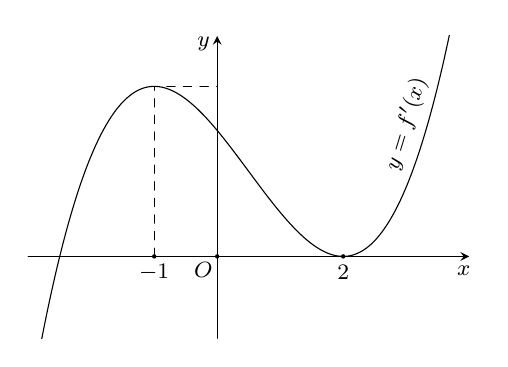
\begin{tikzpicture} [scale=.8, font=\footnotesize, line join=round, line cap=round, >=stealth]
\def \xmin{-3}\def \xmax{4}\def \ymin{-1.3}\def \ymax{3.5} 
\draw[->] (\xmin,0)--(\xmax,0) node[shift=(-110:0.2)] {$x$};
\draw[->] (0,\ymin)--(0,\ymax) node[shift=(-150:0.2)] {$y$};
\fill (0,0) circle(1pt) node[shift=(-135:0.25)]{$O$}
 (-1,0) circle(1pt) node[shift=(-90:0.2)]{$-1$}
 (2,0) circle(1pt) node[shift=(-90:0.2)]{$2$};
\clip (\xmin,\ymin) rectangle (\xmax,\ymax); 
\draw[yscale=0.2, smooth,samples=100,domain=\xmin:\xmax] plot(\x, {(\x)^3-1.5*(\x)^2-6*(\x)+10});
 \draw[dashed] (-1,0)--(-1,2.7)--(0,2.7);
 \draw (3,2.1) node[rotate=73]{$y=f'(x)$};
 \end{tikzpicture}
 }
 \shortans{1}
 \loigiai{
 Số điểm cực trị của hàm số đã cho là $1$. Vì dựa vào đồ thị của $f'(x)$ ta thấy $f'(x)$ đổi dấu một lần từ âm sang dương nên hàm số đã cho có một cực trị (một cực tiểu).
 }
\end{ex}

\begin{ex}%[2-D1B5-SO-15-2425]%[VN-MT-7, Đoàn Thị Lý]%[2D1H4-1]
 Tiệm cận xiên của đồ thị hàm số $y=f(x)=\dfrac{x^2-x+1}{x-1}$ có dạng $y=a x+b,(a, b \in \mathbb{Z})$. Tính giá trị biểu thức $P=5 a+2024 b$.
 \shortans{5}
 \loigiai{
 Giả sử hàm số có đồ thị là $(C)$. Ta có $y=\dfrac{x^2-x+1}{x-1}=x+\dfrac{1}{x-1}$. Từ đó có
 \[\lim\limits _{x \to \pm \infty}[f(x)-x]=\lim\limits _{x \to \pm \infty}\left[\dfrac{x^2-x+1}{x-1}-x\right]=\lim\limits _{x \to \pm \infty} \dfrac{1}{x-1}=\lim\limits _{x \to \pm \infty} \dfrac{\dfrac{1}{x}}{1-\dfrac{1}{x}}=0.\] 
 Suy ra $(C)$ có tiệm cận xiên là đường thẳng $y=x$.\\
 Vậy $a=1$, $b=0$, $P=5a+2024 b=5\cdot 1+2024\cdot 0=5$.
 }
\end{ex}

\begin{ex}%[2-D1B5-SO-15-2425]%[VN-MT-7, Đoàn Thị Lý]%[2D1V1-3]
 Cho hàm số $y=f(x)$ có đạo hàm trên $\mathbb{R}$ và bảng xét dấu đạo hàm như hình vẽ sau:
 \begin{center}
 
\begin{tikzpicture}
 \tkzTabInit[nocadre=true,lgt=1.2,espcl=2.5,deltacl=0.5]
 {$x$ /.7, $f'(x)$ /.7}
 {$-\infty$,$-10$,$-2$,$3$,$8$,$+\infty$}
 \tkzTabLine{ ,+,0,+,0,-,0,-,0,+, }
 \end{tikzpicture}
 \end{center} 
 Tìm $m$ để hàm số $y=f\left( x^3+4x+m \right)$ nghịch biến trên khoảng $(-1;1)$?
 \shortans{3}
 \loigiai{
 Đặt $t=x^3+4x+m\Rightarrow t'=3x^2+4>0,\,\forall x\in (-1;1)$ nên $t$ đồng biến trên $(-1;1)$ và $t\in \left(m-5;m+5\right)$.\\
 Yêu cầu bài toán trở thành tìm $m$ để hàm số $f(t)$ nghịch biến trên khoảng $\left( m-5;m+5 \right)$.\\
 Dựa vào bảng xét dấu ta được $\heva{& m-5\ge -2 \\ 
 & m+5\le 8}\Leftrightarrow \heva{& m\ge 3 \\ 
 & m\le 3}\Leftrightarrow m=3$.
 }
\end{ex}

\begin{ex}%[2-D1B5-SO-15-2425]%[VN-MT-7, Đoàn Thị Lý]%[2D1V1-3]
 \immini{
 Cho hàm số $y=f(x)$ có đạo hàm liên tục trên $\mathbb{R}$ và có đồ thị $y=f'(x)$ như hình vẽ bên. Đặt $g(x)=f(x-m)-\dfrac{1}{2}{(x-m-1)^2}+2019$, với $m$ là tham số thực. Gọi $S$ là tập hợp các giá trị nguyên dương của $m$ để hàm số $y=g(x)$ đồng biến trên khoảng $(5;6)$. Tính tổng tất cả các phần tử thuộc $S$.
 }
 {
 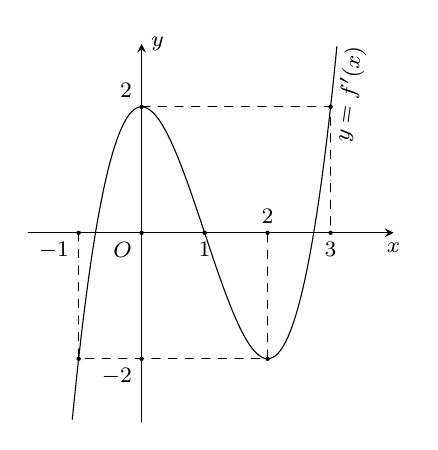
\begin{tikzpicture} [scale=.8, font=\footnotesize, line join=round, line cap=round, >=stealth]
 \draw[->] (-1.8,0)--(0,0) node[below left]{$O$}--(4,0) node[below]{$x$};
 \draw[->] (0,-3)--(0,3) node[right]{$y$};
 \draw[samples=100,domain=-1.1:3.1,smooth] plot (\x, {(\x)^3-3*(\x)^2+2});
 \draw[dashed] (-1,0) node[below left]{$-1$}--(-1,-2)--(0,-2)node[below left]{$-2$}--(2,-2)--(2,0)node[above]{$2$} (0,2)node[above left]{$2$}--(3,2)--(3,0) node[below]{$3$};
 \draw (1,0) node[below] {$1$};
 \foreach \i in {(0,0),(3,2),(2,-2),(0,2),(-1,-2),(-1,0),(2,0),(0,-2),(1,0),(3,0)}\fill \i circle (1pt);
 \draw (3.3,2.2) node[rotate=82]{$y=f'(x)$};
 \end{tikzpicture}
}
 \shortans{14}
 \loigiai{
 Ta có 
 $g'(x)=f'(x-m)-(x-m-1)$.\\
 Xét phương trình $g'(x)=0\Leftrightarrow f'(x-m)-(x-m-1)=0\qquad (1)$.\\
 Đặt $x-m=t$, phương trình (1) trở thành $f'(t)-(t-1)=0\Leftrightarrow f'(t)=t-1\qquad(2)$.\\
 Nghiệm của phương trình $(2)$ là hoành độ giao điểm của hai đồ thị hàm số $y=f'(t)$ và $y=t-1$.\\
 Ta có đồ thị các hàm số $y=f'( t)$ và $y=t-1$ như sau: 
 \begin{center}
 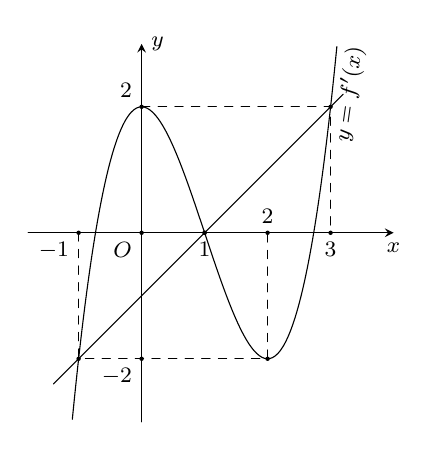
\begin{tikzpicture} [scale=.8, font=\footnotesize, line join=round, line cap=round, >=stealth]
 \draw[->] (-1.8,0)--(0,0) node[below left]{$O$}--(4,0) node[below]{$x$};
 \draw[->] (0,-3)--(0,3) node[right]{$y$};
 \draw[samples=100,domain=-1.1:3.1,smooth] plot (\x, {(\x)^3-3*(\x)^2+2});
 \draw[samples=100,domain=-1.4:3.2,smooth] plot (\x, {(\x)-1});
 \draw[dashed] (-1,0) node[below left]{$-1$}--(-1,-2)--(0,-2)node[below left]{$-2$}--(2,-2)--(2,0)node[above]{$2$} (0,2)node[above left]{$2$}--(3,2)--(3,0) node[below]{$3$};
 \draw (1,0) node[below]{$1$};
 \foreach \i in {(0,0),(1,0),(3,2),(2,-2),(0,2),(-1,-2),(-1,0),(2,0),(0,-2),(1,0),(3,0)}\fill \i circle (1pt);
 \draw (3.3,2.2) node[rotate=82]{$y=f'(x)$};
 \end{tikzpicture}
 \end{center} 
 Căn cứ đồ thị các hàm số ta có phương trình (2) có nghiệm là $\hoac{& t=-1 \\ 
 & t=1 \\ 
 & t=3 }
 \Rightarrow\hoac{&x=m-1 \\ 
 & x=m+1 \\ 
 & x=m+3.}$\\
 Ta có bảng biến thiên của $y=g(x)$ như sau:
 \begin{center}
 
\begin{tikzpicture}
 \tkzTabInit[nocadre=true,lgt=1.2,espcl=2.5,deltacl=0.5]
 {$x$/0.7,$g’(x)$/0.7,$g(x)$/2}
 {$-\infty$,$m-1$,$m+1$,$m+3$,$+\infty$}
 \tkzTabLine{,-,0,+,0,-,0,+,}
 \tkzTabVar{+/$+\infty$,-/,+/,-/,+/$+\infty$}
 \end{tikzpicture}
 \end{center}
 Để hàm số $y=g(x)$ đồng biến trên khoảng $(5;6)$ cần 
 $\hoac{
 & \heva{
 & m-1\le 5 \\ 
 & m+1\ge 6} \\ 
 & m+3\le 5 \\ }\Leftrightarrow \hoac{
 & 5\le m\le 6 \\ 
 & m\le 2.}$\\
 Vì $m\in \mathbb{N}^*$ nên $m\in \big\{1;2;5;6\big\}$. Suy 
 $S=14$.
 }
\end{ex}

\begin{ex}%[2-D1B5-SO-15-2425]%[VN-MT-7, Đoàn Thị Lý]%[2D1V3-6]
 Một hộp sữa dung tích $1 \ell$ (lít) có dạng hình hộp chữ nhật với đáy là hình vuông cạnh bằng $x$ cm và chiều cao $h$ cm. Tìm giá trị của $x$ để diện tích toàn phần của hình hộp là nhỏ nhất.
 \shortans[]{10}
 \loigiai{
 \begin{center}
 \begin{tikzpicture}
 \def\a{3}
 \def\b{2}
 \def\g{30}
 \def\h{2}
 \path
 (0:0) coordinate (A)--++(\g:\b) coordinate (B)--++(0:\a) coordinate (C)--++(\g-180:\b) coordinate (D)
 \foreach \x in {A,B,C,D}{
 ($(\x)+(90:\h)$) coordinate (\x')}
 ;
 \foreach \x/\g in {A/180,B/150,C/0,D/-30,A'/180,B'/150,C'/0,D'/-30}
 \fill[black](\x) circle (1pt);
 \draw[dashed] (B')--(B)--(A)
 (B)--(C);
 \draw
 (A)--(D)--(D')--(A')--cycle
 (A')--(B')--(C')--(D')
 (D)--(C)--(C');
 \draw (1.6,0.15) node {$x$} (4,.4) node {$x$} (5,2) node {$h$}
 ;
 \end{tikzpicture} 
 \end{center}
 Thể tích của hộp sữa là $V=x^2h$ $\mathrm{cm}^3$.\\
 Theo bài ra, ta có $V=1\mathrm{\ell}=1000 \mathrm{\,cm}^3$. Suy ra $x^2h=1000\Rightarrow h=\dfrac{1000}{x^2}$.\\
 Ta có diện tích toàn phần của hộp sữa là \[S_{\rm{tp}}=S_{\rm{xq}}+S_{\rm{d}}=4hx+2x^2=4\cdot\dfrac{1000}{x^2}\cdot x+2x^2=2x^2+\dfrac{4000}{x}.\]
 Đặt $y=f(x)=2x^2+\dfrac{4000}{x}$, suy ra $f'(x)=4x-\dfrac{4000}{x^2}$.\\
 Xét $f'(x)=0\Leftrightarrow 4x-\dfrac{4000}{x^2}=0\Leftrightarrow 4x^3-4000=0\Leftrightarrow x=10$.\\
 Ta có bảng biến thiên của hàm số $y=f(x)$ như sau:
 \begin{center}
 
\begin{tikzpicture}
 \tkzTabInit[nocadre=true,lgt=1.2,espcl=2.5,deltacl=0.5]
 {$x$/0.7,$f’(x)$/0.7,$f(x)$/2}
 {$0$,$10$,$+\infty$}
 \tkzTabLine{d,-,0,+,}
 \tkzTabVar{-D+//$+\infty$,-/$600$,+/$+\infty$}
 \end{tikzpicture}
 \end{center}
 Vậy để hộp sữa có diện tích toàn phần nhỏ nhất thì $x=10$.
 } 
\end{ex}
\Closesolutionfile{ans}
% \begin{indapan}
% 	{ans/ans\currfilebase}
% \end{indapan}

